
\chapter{Background}
\label{chap:background}

We introduce in this chapter the most important concepts and methods employed in the field of spoken dialogue systems, with special emphasis on dialogue management.  We start by describing some key linguistic concepts that are particularly relevant for our work: turn-taking, dialogue acts and grounding.  A proper understanding of these aspects is indeed a prerequisite for the design of conversationally competent dialogue systems. After this linguistic overview, we move to a more technical discussion of the software architectures used to implement practical dialogue systems.  These architectures typically comprise multiple processing components, from speech recognition to understanding, dialogue management, output generation and speech synthesis.  We briefly describe the role of each component and their positions in the global processing pipeline. 

Last but not least, the final section of this background chapter delves into the diverse set of approaches that have been explored in the technical literature to formalise the dialogue management problem.  We first present hand-crafted approaches, starting with finite-state policies and pursuing with more sophisticated methods based on logic- or plan-based reasoning.  Finally, we detail the more recently developed statistical approaches to dialogue management that aim to automatically extract dialogue strategies from interaction data.

\section{What is spoken dialogue?}

We communicate in order to fulfil a wide array of social functions, such as exchanging ideas, recollecting experiences,  sustaining relationships, or collaborating with others to accomplish shared goals. These communication skills are developed in early childhood, and our cognitive abilities are in many ways shaped and amplified by this disposition for verbal interaction.  

One of the most important property of dialogue is that it is fundamentally a \textit{collaborative activity} (emphasis on both terms).  It is, first of all, an \textit{activity}, which means that is is (1) driven by (practical and/or social) goals to achieve; (2) subject to costs that should be minimised -- the communication effort --, and (3) composed of a temporal sequence of basic actions.  Furthermore, if we abstract from so-called ``internal dialogues'' with oneself, dialogue involves per definition at least two participants that must act together to keep the dialogue running.  As shown by a wealth of studies in psychology and linguistics \citep{Clark1989,Allwood92,Clark96,Garrod2004,Tomasello2005}, human conversations are characterised by a high degree of \textit{collaboration} between interlocutors.  The individuals participating in a dialogue routinely collaborate in order to coordinate their contributions and ensure mutual understanding, thereby making the interaction more efficient. This collaboration is done mostly unconsciously and is part and parcel of the conversational skills we develop as speakers of a given language. 

We describe in the next sections four major aspects of this collaborative activity: \begin{enumerate}
\item The dialogue participants take \textit{turns} in a conversation;
\item These turns are structured into basic communicative units called \textit{dialogue acts};
\item The interpretation of these dialogue acts is subordinated to the \textit{conversational context} in which they are uttered ; 
\item The participants continuously provide \textit{grounding signals} to each other in order to indicate how they understand (or fail to understand) their contributions.
\end{enumerate}

\subsection{Turn-taking}

Turn-taking\index{turn-taking} is one of the most basic (yet often neglected) aspect of spoken dialogue. The physical constraints of the communication channel impose that participants take turns in order to speak.   Turn-taking is essentially a resource allocation problem.  In this case, the resource to allocate is called the conversational floor\index{conversational floor}, and social conventions dictate how the dialogue participants are to take and release their turns. 

The field of  \textit{conversation analysis}\index{conversation analysis} studies what these conventions are and how they combine to shape conversational behaviours in various languages and cultures. Human conversations are indeed remarkably efficient at turn-taking.  Empirical cross-linguistic studies have shown that the average transition time between turns revolves around 250 ms. \citep{Stivers30062009}.\footnote{Interestingly, this duration is shorter than the time required for a human speaker to plan the motor routines associated with the physical act of speaking.  This means that the next speaker must start planning his utterance before the current turn is complete, and predict when a potential turn boundary is likely to appear.} In addition, most of the utterances do not overlap: \cite{Levinson1983} argues that less than 5 \% of the speech stream contains some form of overlap in spontaneous conversations.  

A wide variety of cues are used to detect turn boundaries, such as silence, hesitation markers, syntax (complete grammatical unit), intonation (rising or falling pitch) and body language, as detailed by \cite{Duncan1972}.   These cues can occur jointly or in isolation. Upon reaching a turn boundary, a set of social conventions govern who is allowed to take the turn.  The current speaker can explicitly select the next person to take the turn, for instance when greeting someone or asking a directed question \citep{sacks1974}.   This selection can also occur via other mechanisms such as gaze.  When no such selection is indicated, other participants are allowed to take the turn.  Alternatively, the current speaker can continue to hold the floor until the next boundary. 

Turn-taking is closely related to the notion of \textit{initiative}\index{initiative} in research on human--computer interaction. The vast majority of dialogue systems currently deployed are either system-initiated or user-initiated.  In a system-initiated dialogue, the dialogue system has full control on how the interaction is unfolding -- i.e. the system is the one asking the questions and waiting for the user responses.  A user-initiated dialogue is the exact opposite: in such settings, the user is assumed to lead the interaction and request information from the system.  The most complex -- but also most natural -- interaction style is the mixed-initiative\index{mixed initiative}, where both the user and the dialogue system are allowed to take the initiative at any time and decide to either provide or solicit information whenever they see fit \citep{Horvitz:1999}. 

The turn-taking behaviour of most current-day dialogue systems remains quite rudimentary.  The most common method to detect the end of a user turn is to wait for a silence longer than a manually fixed threshold, typically ranging between 
\textonehalf  $ $ and 1.0 second.  Some system architectures also include routines for handling barge-ins\index{barge-in} -- that is, user interruptions --  \citep{StromS00}, while others simply ignore them altogether . Turn-taking has now become a focus of research in its own right in the dialogue system literature \citep{RauxE09,Gravano2011}, in an effort to break away from the ping-pong interaction style that characterises most current dialogue interfaces.  

\subsection{Dialogue acts}

Each turn is constituted of one or more utterances.  As argued by \cite{Austin1962} and \cite{Searle1969}, our utterances are nearly always purposeful: they have specific goals and are intended to provoke a specific psychological effect on the listener(s).  They should therefore best be described as actions rather than abstract statements about the world.  The notion of dialogue act\index{dialogue act} embodies precisely this idea.\footnote{Dialogue acts have gone through multiple names over time, owing to the diverse range of research fields that have studied them, from philosophy to descriptive and computational linguistics.  As listed in \cite{mctear2004}, alternative denominations include speech acts \citep{Searle1969}, communicative acts \citep{allwood1976}, conversation acts \citep{TraumH92}, conversational moves \citep{sinclair1975}, and dialogue moves \citep{LarssonCEL99}.} \cite{Bunt1996} defines a dialogue act as a ``functional unit of a dialogue used by the speaker to change the context''.

In his seminal work on the philosophy of language, \cite{Searle1979} established a taxonomy of speech acts\index{speech act} divided in five central categories:
\begin{description}
\item[Assertives: ] Committing the speaker to the truth of a proposition. \\
Examples: \utt{I swear I saw him on the crime scene.}, \utt{I bought more coffee.}
\item[Directives: ]  Attempts by the speaker to get the addressee to do something. \\ Examples:  \utt{Clean your room!}, \utt{Could you post this for me?}
\item[Commissives: ] Committing the speaker to some future course of action. \\ Examples: \utt{I will deliver this review before Monday.}, \utt{I promise to work on this.}
\item[Expressives: ] Expressing the psychological state of the speaker about a state of affairs. \\ Examples: \utt{I am so happy for you!}, \utt{Apologies for being late.}
\item[Declaratives: ] Bringing about a different state of the world by the utterance. \\ Examples: \utt{You're fired.}, \utt{We decided to let you pass this exam.}
\end{description}

Modern taxonomies of dialogue acts are significantly more detailed than the one introduced by Searle.  They also provide detailed accounts of various dialogue-level phenomena such as grounding (cf. next section) that were absent from Searle's analysis. The most well-known annotation scheme is DAMSL (Dialogue Act Markup in Several Layers\index{DAMSL}), which was initially put forward by \cite{Core1997}.  DAMSL defines a rich, multi-layered annotation scheme for dialogue acts that is both domain- and task- independent.  A modified version of this scheme was applied to annotate the Switchboard corpus\footnote{The Switchboard corpus is a corpus of spontaneous telephone conversations collected in the early 1990's.  It includes about 2430 conversations averaging 6 minutes in length; totalling over 240 hours of recorded speech with native speakers of American English \citep{Godfrey1992}.} based on a set of 42 distinct dialogue acts \citep{Jurafsky1997}, including greeting and closing actions, acknowledgements, clarification requests, self-talk, responses, and many more.  An interesting aspect of DAMSL is the use of two complementary dimensions in the markup: the \textit{forward-looking functions}\index{forward-looking function}, which are the traditional speech acts in Searle's sense (assertions, directives, information requests, etc.) and the \textit{backward-looking functions}\index{backward-looking function} that respond back to a previous dialogue act and can signal agreement, understanding, or provide answers.  Both backward- and forward-looking functions can be present in the same utterance. 

Determining the dialogue act corresponding to a given utterance is a non-trivial operation. The type of utterance only gives a partial indication of the underlying dialogue act -- a question can for instance express a directive (\utt{Could you post this for me?}).  In order to accurately classify a dialogue act, a variety of linguistic factors have to be taken into account, such as prosody, lexical, syntactic and semantic features, and the preceding dialogue history \citep{jurafsky1998,Shriberg1998,stolcke2000,Keizer2007}.

\subsection{Interpretation of dialogue acts} 

Dialogue acts are strongly contextual in nature: their precise meaning can often only be comprehended within the particular conversational context in which they appear. The successful interpretation  of dialogue acts must therefore venture beyond the boundaries of the isolated utterance. We briefly review here three striking aspects of this dependence on context.

\subsubsection*{Implicatures}
\index{implicature}
As shown by \cite{Grice1989}, an important part of the semantics of dialogue acts is not explicitly stated but rather implied from the context.  Consider the following constructed example: 
\begin{center}
\begin{dialogue}
\speak{A} Is William working today?
\speak {B} He has a cold.
\end{dialogue}
\end{center}
In order to retrieve the ``suggested'' meaning behind B's utterance -- namely, that William is probably not working --, one needs to assume that B is cooperative and that his response is therefore relevant to A's question.  If an utterance initially seems to deliberately violate this principle, the listener must search for additional hypotheses required to make sense of the dialogue act. \cite{Grice1989} formalised these ideas in terms of a cooperative principle composed of four conversational maxims that are assumed to hold in a natural conversation: the maxim of quality (``be truthful''), the maxim of quantity (``be exactly as informative as required''), the maxim of relation (``be relevant'') , and the maxim of manner (``be relevant'').  These notions have been further developed by various theorists such as \cite{wilson2002relevance} and \cite{horn2008handbook}.  A computational account of these implicatures (and application to dialogue systems) is provided by \cite{benotti2010implicature}. 


\subsubsection*{Non-sentential utterances}
\label{non-sentential utterance}
\index{non-sentential utterance}
Non-sentential (also called elliptical) utterances are linguistic constructions that lack an overt predicate.  They include expressions such as  \utt{where?}, \utt{at 8 o'clock}, \utt{a bit less, thanks} and \utt{brilliant!}. Their interpretation generally requires access to the recent dialogue history to recover their intended meaning. This can lead to ambiguities in the resolution, as illustrated in these examples modified from \cite{Fernandez:2007}: \begin{itemize}
\item A: ``When do they open the new station?''  $\rightarrow$ B: ``Tomorrow'' (\textit{short answer})
\item A: ``They open the station today''  $\rightarrow$ B: ``Tomorrow'' (\textit{correction})
\item A: ``They open the station tomorrow''  $\rightarrow$ B: ``Tomorrow'' (\textit{acknowledgement})
\end{itemize}

Various accounts of non-sentential utterances have been proposed, based on e.g. discourse coherence \citep{Schlangen03theinterpretation} or interaction-oriented semantics \citep{fernandez2006non,Ginzburg2012}. Machine learning approaches have also been developed \citep{Schlangen:2005,Fernandez:2007}. 

\subsubsection*{Referring expressions}

Finally, dialogue acts are replete with linguistic expressions that refer to some aspect of the conversational context.  These references can be either deictic or anaphoric. 

A deictic marker\index{deictic marker} is a reference to an entity that is determined by the context of enunciation.  Examples of such markers are \utt{here} (spatial reference), \utt{yesterday} (temporal reference), \utt{this mug} (demonstrative), \utt{you} (reference to a person), or even pointing gestures. By their very definitions, deictic markers refer to different realities depending on the situation in which they are used: a \utt{here} uttered in a classroom differs from a \utt{here} uttered in the countryside.  

In addition, dialogue can also include anaphoric expressions -- that is, expressions that refer to an element that has been previously mentioned through the history of the dialogue. An simple example of such anaphoric expression can be seen in the question-answer pair \utt{Is William working today?} $\rightarrow$ \utt{He has a cold}, where the pronoun \utt{he} must be resolved to \utt{William}. 

The appropriate processing of deictic and anaphoric expressions is an important question in dialogue systems, and pertains both to the interpretation and production process. Multiple approaches have been pursued, relying on symbolic \citep{Eckert2000} or statistical techniques \citep{StrubeM03,Stent2010}.  Researchers have also investigated the integration of salience measures \citep{Kelleher:2004}, multimodal cues \citep{Frampton:2009,Chen:2011}, the processing of spatial referring expressions \citep{zender/etal:2009-ijcai} and the incrementality of the resolution process \citep{schlangen2009incremental,poesio2011incremental}. 

\subsection{Grounding}

Dialogue acts are executed as part of a larger collaborative activity that requires the active coordination of all conversational partners, i.e. speaker(s) as well as hearer(s).  This coordination takes place at various levels.  The first and most visible level is the content of the conversational activity.   The partners must ensure mutual understanding of each other's contribution, to control that they remain ``on the same page''.  In addition, they  also coordinate the process by which the conversational activity moves forward -- by signalling that they are attending to the person who currently holds the conversational floor and acknowledging his/her contributions to the dialogue.

As an illustration, consider this short excerpt from a real conversation transcribed in the British National Corpus \citep{bnc} :

\begin{dialogue} 
\speak{Kathleen } How come they can take time off yet you can't?
\speak{Steve } $\ \ \ \ \ \ $ He's been there longer than me.
\speak{Kathleen } Oh.
\speak{Steve }  $\ \ \ \ \ \ $ I can, I might have two holidays now, two days' holiday. ...
\speak{Kathleen } Well ... I don't get that, me.
\speak{Steve }  $\ \ \ \ \ \ $ What?
\speak{Kathleen } All these two days' holiday and this, you've had Christmas.
\speak{Steve }  $\ \ \ \ \ \ $ You get two point summat\footnote{``Summat'' is slang for ``something'' in the Yorkshire region. } days per month worked
\speak{Kathleen } Oh so you should've got them for January? ...
\speak{Steve }  $\ \ \ \ \ \ $ right?
\speak{Kathleen } Yeah.
\speak{Steve }  $\ \ \ \ \ \ $ And I worked three month before Christmas so I got six point summat days
\speak{Kathleen } For Christmas.
\speak{Steve }  $\ \ \ \ \ \ $ so then I had all Christmas off.
\speak{Kathleen } Oh! \\
 $\phantom{a} \ \ \ \ \ \ \ $ Yeah I get it now. \\
 $\phantom{a} \ \ \ \ \ \ \ $ ... I thought you got Christmas off like we got Christmas off.
\speak{Steve }  $\ \ \ \ \ \ $ No. \\ 
 $\phantom{a} \ \ \ \ \ \ \ $ You gotta earn them. ... \vspace{-2mm}
 \begin{flushright}\begin{scriptsize}(\urlsmall{http://www.phon.ox.ac.uk/SpokenBNCdata/KCX.html})\end{scriptsize}\end{flushright} 
\end{dialogue} 

We can observe in this short dialogue that the interlocutors constantly rely on the \textit{common ground} of the interaction to move their discussion forward.  They regularly check what pieces of information are mutually known and understood (e.g. \utt{right?}).  They also make use of a variety of signals to indicate when things are properly grounded (\utt{oh}, \utt{yeah}, \utt{I get it}) and when they are not (\utt{I don't get that}, \utt{what?}).  As the dialogue unfolds, this common ground\index{common ground} accumulates more and more information -- for instance, the system of holiday entitlement is not initially part of the shared knowledge for both speakers at the onset of the conversation, but becomes so towards the end. 

The common ground is defined as the collection of shared knowledge, beliefs and assumptions that is established during an interaction.\footnote{An information that is part of the common ground for a given group is more than simply known by every member of the group.  They must also be aware that the information is shared and known by the other members. Formally speaking, a proposition $p$ is part of the common knowledge for a group of agents $G$ when all the agents in $G$ know $p$, and they also all know that they all know $p$, and they all know that they all know that they all know $p$, \textit{ad infinitum}. This definition can be rigorously formalised with set theory or epistemic logic \citep{meyer2004epistemic}. } Each dialogue act is built upon the current common ground and participates in its gradual expansion and refinement.  This process is called \textit{grounding}\index{grounding}.  A variety of feedback mechanisms  can be used to this effect.  As described by \cite{Clark1989}, positive evidence\index{positive feedback} of understanding can be expressed via cues such as:
\begin{description}
\item[Continued attention: ] The hearer shows that he/she continues to attend to the speaker;
\item[Relevant next contribution: ] The hearer produces a relevant follow-up, as in the answer \utt{He's been there longer than me} following the question that precedes it;
\item [Acknowledgement: ] The hearer nods or utters a backchannel such as \utt{mm}, \utt{uh-uh}, \utt{yeah}, or an assessment such \utt{I see}, \utt{great}, \utt{I get it now};
\item [Demonstration: ] The hearer demonstrates evidence of understanding by reformulating or completing the speaker utterance;
\item [Display: ] The hearer reuses part of the previous utterance.
\end{description}

Communication problems can also occur, owing to e.g. misheard or misunderstood utterances. The hearer must in this case provide a negative feedback\index{negative feedback} indicating a trouble in understanding.  A large panel of clarification and repair strategies\index{clarification strategy} \index{repair strategy} are available to recover from these communicative failures.  These strategies include backchannels\index{backchannel} (\utt{mm?}), confirmations  (\utt{Do you mean that...?}), requests for disambiguations, invitations to repeat, and tentative corrections.  

All in all, these positive and negative signals enable the dialogue participants to dynamically synchronise what the speaker intends to express and what the hearers actually understand.   This grounding process operates mostly automatically, without deliberate effort.  It is closely related to the concept of interactive alignment\index{alignment} that has recently been articulated by \cite{Garrod2004,Garrod2009}. Humans show a clear tendency to (unconsciously) imitate their conversational partners. In particular, they automatically align their choice of words, a phenomenon called lexical entrainment\index{lexical entrainment} \citep{brennan1996conceptual}.  But alignment also occurs on several other levels such as grammatical constructions \citep{branigan2000syntactic}, pronunciation \citep{pardo2006phonetic}, accents and speech rate \citep{giles19911}, and even gestures and facial expressions \citep{bavelas1986show}.  

A proper treatment of grounding is critical for the development of conversational interfaces.  As we already mentioned in the introduction to this thesis, understanding errors are indeed ubiquitous in spoken dialogue systems.  The potential sources of misunderstandings are abundant, from error-prone speech recognition to out-of-domain utterances, unresolved ambiguities, and unexpected user behaviour.  Appropriate grounding strategies are crucial to address these pitfalls. Grounding for dialogue systems is an active area of research and important advances have been made regarding the formalisation of rich computational models of grounding \citep{Traum:1994thesis,MathesonPT00}, the generation of clarification requests \citep{Purver04Thesis,Rieser:2005}, the design of human-inspired error handling\index{error handling} strategies \citep{Skantze2007}, the integration of non-verbal cues such as gaze, head nods and attentional focus \citep{Nakano:2003}, and the development of incremental grounding mechanisms \citep{visser_toward_2012}.

\section{Spoken Dialogue Systems}

After reviewing some of the core properties of human dialogues, we now discuss how to develop practical computer systems that can emulate (to a limited extent) such conversational behaviour.   In the previous chapter, Figure \ref{fig:basicsds} represented a dialogue system as a black box taking speech inputs from the user and generating spoken responses.   Real systems have however a complex internal structure, as we describe in the next pages.

 \subsection{Architectures}

Spoken Dialogue Systems (SDS) often take the form of complex software architectures\index{dialogue system architectures} that encompass a wide range of interconnected components. These components are dedicated to various tasks related to speech processing, understanding, reasoning and decision-making. Upon perceiving a new speech signal from the user, these tasks can be grouped in five consecutive steps: 
\begin{enumerate}
\item \textit{Speech recognition}, in charge of mapping the raw speech signal to a set of recognition hypotheses for the user utterance(s);
\item \textit{Speech understanding}, in charge of mapping the recognition hypotheses to high-level semantic representations of the dialogue act performed by the user;
\item \textit{Dialogue management}, in charge of interpreting the purpose of the dialogue act in the larger dialogue context, and then deciding what communicative action to perform (if any);
\item \textit{Generation}, in charge of finding the best linguistic (and extra-linguistic) realization for the selected communicative action;
\item And finally, \textit{text-to-speech synthesis}, in charge of synthesizing an audio signal out of the generated utterance.
 \end{enumerate}
 \index{speech recognition}\index{dialogue understanding}\index{dialogue management}\index{natural language generation}\index{text-to-speech synthesis}
 
 Figure \ref{fig:architecture} shows the flow of information for a prototypical spoken dialogue system.  The schema only provides an abstract, simplified view of the global architecture.  Depending on the practical needs of the application, many systems will deviate from this schema through the removal, modification or addition of various modules.  It should also be noted that many systems rely on additional middleware to act as a ``software glue'' between the components and handle various tasks related to the flow of information and scheduling of modules \citep{jaspis2004,Herzog:2004,Bohus:2009,schlangen2010}.
   
 \begin{figure}[h]
\centering
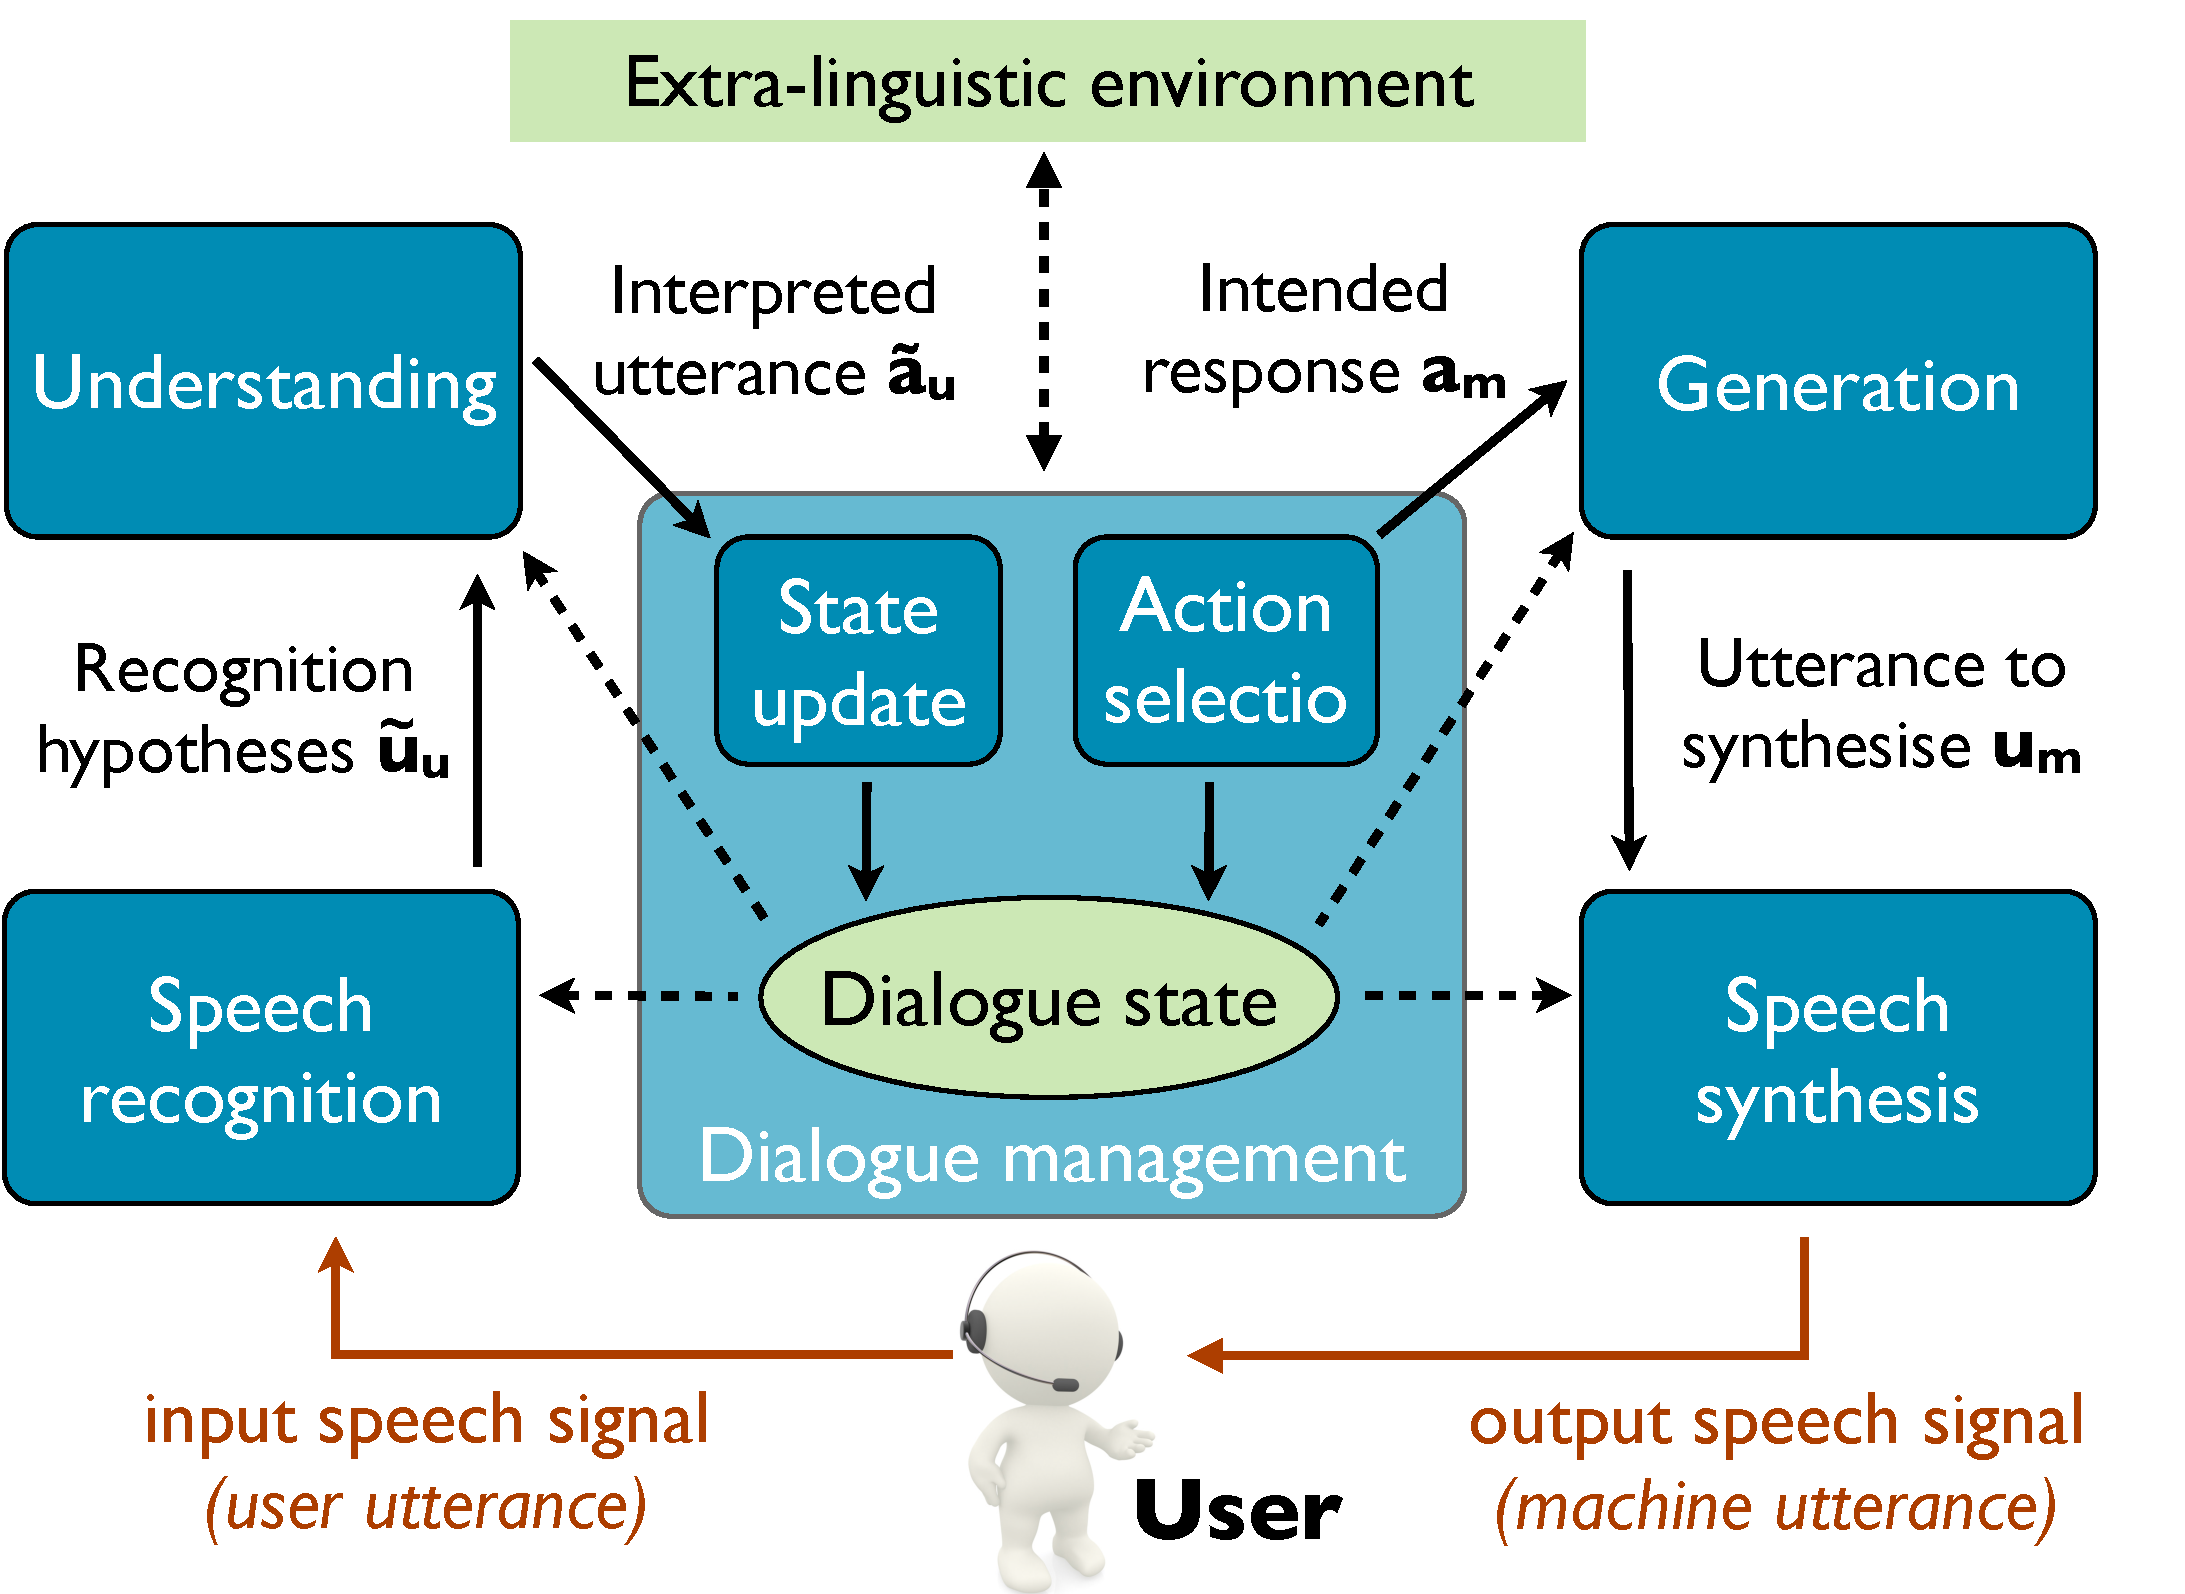
\includegraphics[scale=0.32]{imgs/architecture.pdf}
\caption{Information flow for a typical spoken dialogue system. The solid lines denote necessary input and outputs while the dotted lines represent optional contextual information.}
\label{fig:architecture}
\end{figure}

Spoken dialogue systems can rely on other modalities than speech.  In particular, additional communication channels such as touch, gestures, gaze, and other body movements can be fruitfully exploited.  As shown in eg. \cite{smartkom}, multiple modalities can be used to enrich communication in both directions (understanding and generation). \index{multi-modality}\index{multi-modal dialogue system}In particular, the system can refine its understanding of the actual user intentions by fusing information perceived through multiple information channels such as gestures \citep{stiefelhagen2004} or gaze \citep{koller2012}.  Non-verbal modalities can also be exploited to enhance how information is presented back to the user and convey additional grounding signals, through e.g. facial expressions and gestures. It has been notably shown that the use of multiple modalities can reduce understanding errors and cognitive load \citep{oviatt2004we} as well as improve the overall user experience   \citep{JokinenH06}.  For all its advantage, multi-modality poses however a number of additional challenges related to timing and synchronisation \citep{DBLP:conf/hri/SalemKJ13}, interpretation of non-verbal signs \citep{cassell2007trading}, and increased system complexity. 

In addition to the mutiple communication modalities, most dialogue domains also include an external context that must also be accounted for\index{contextal awareness}\index{contextual modelling}.  This external context might be a physical environment, as in human-robot interaction \citep{goodrich2007human}, a virtual world, as for embodied virtual agents \citep{kopp2003max}, a spatial location, as in in-car navigation systems, or simply a database of factual knowledge, as in information systems. Contextual factors of relevance for the application must be continuously monitored by the dialogue system (and updated whenever necessary), as many components depend on the availability of such context model for their internal processing.  Furthermore, the agent can often actively influence this context through external actions (for instance, a grasping action will modify the location of the gripped object).   This contextual awareness necessitates the integration of additional functionalities for perception and actuation into the dialogue system. In human--robot interaction\index{human--robot interaction} domains, these extra-linguistic modules can notably include subsystems for object and scene recognition, spatial navigation, and various motor routines for locomotion and manipulation  \citep{1570637,HawesSWZJKBBS07}. 

Several types of architectures have been proposed to assemble these components in a unified framework.  The simplest approach is to arrange the components sequentially in a pipeline\index{pipeline architecture} starting from speech recognition and ending with speech synthesis.  This approach, although relatively straightforward to develop, has a number of shortcomings, amongst which the rigidity of the information flow and the difficulty of inserting feedback loops between components. Pipelines also offer poor turn-taking capabilities, since the system is unable to react before the pipeline has been fully traversed \citep{RauxE09}. More advanced architectures -- including the one put forward in this thesis -- are based on the notion of \textit{information state}\index{information state} \citep{larsson2000information,bos2003dipper}.  These approaches are essentially blackboard architectures revolving around a central dialogue state that is read and written by various modules connected to it.  These modules listen to the state for relevant changes, in which case they trigger their processing routines and update the state with the result.  The main advantages of such architectures are (1) a more flexible information flow, since the modules are allowed to process and update information in any order, and (2) the possibility to define modules that take full advantage of the contextual information encoded in the dialogue state.  Figure \ref{fig:architecture_comp} provides a graphical illustration of the difference between pipeline and information-state-based architectures.  

 \begin{figure}[h!]
\centering
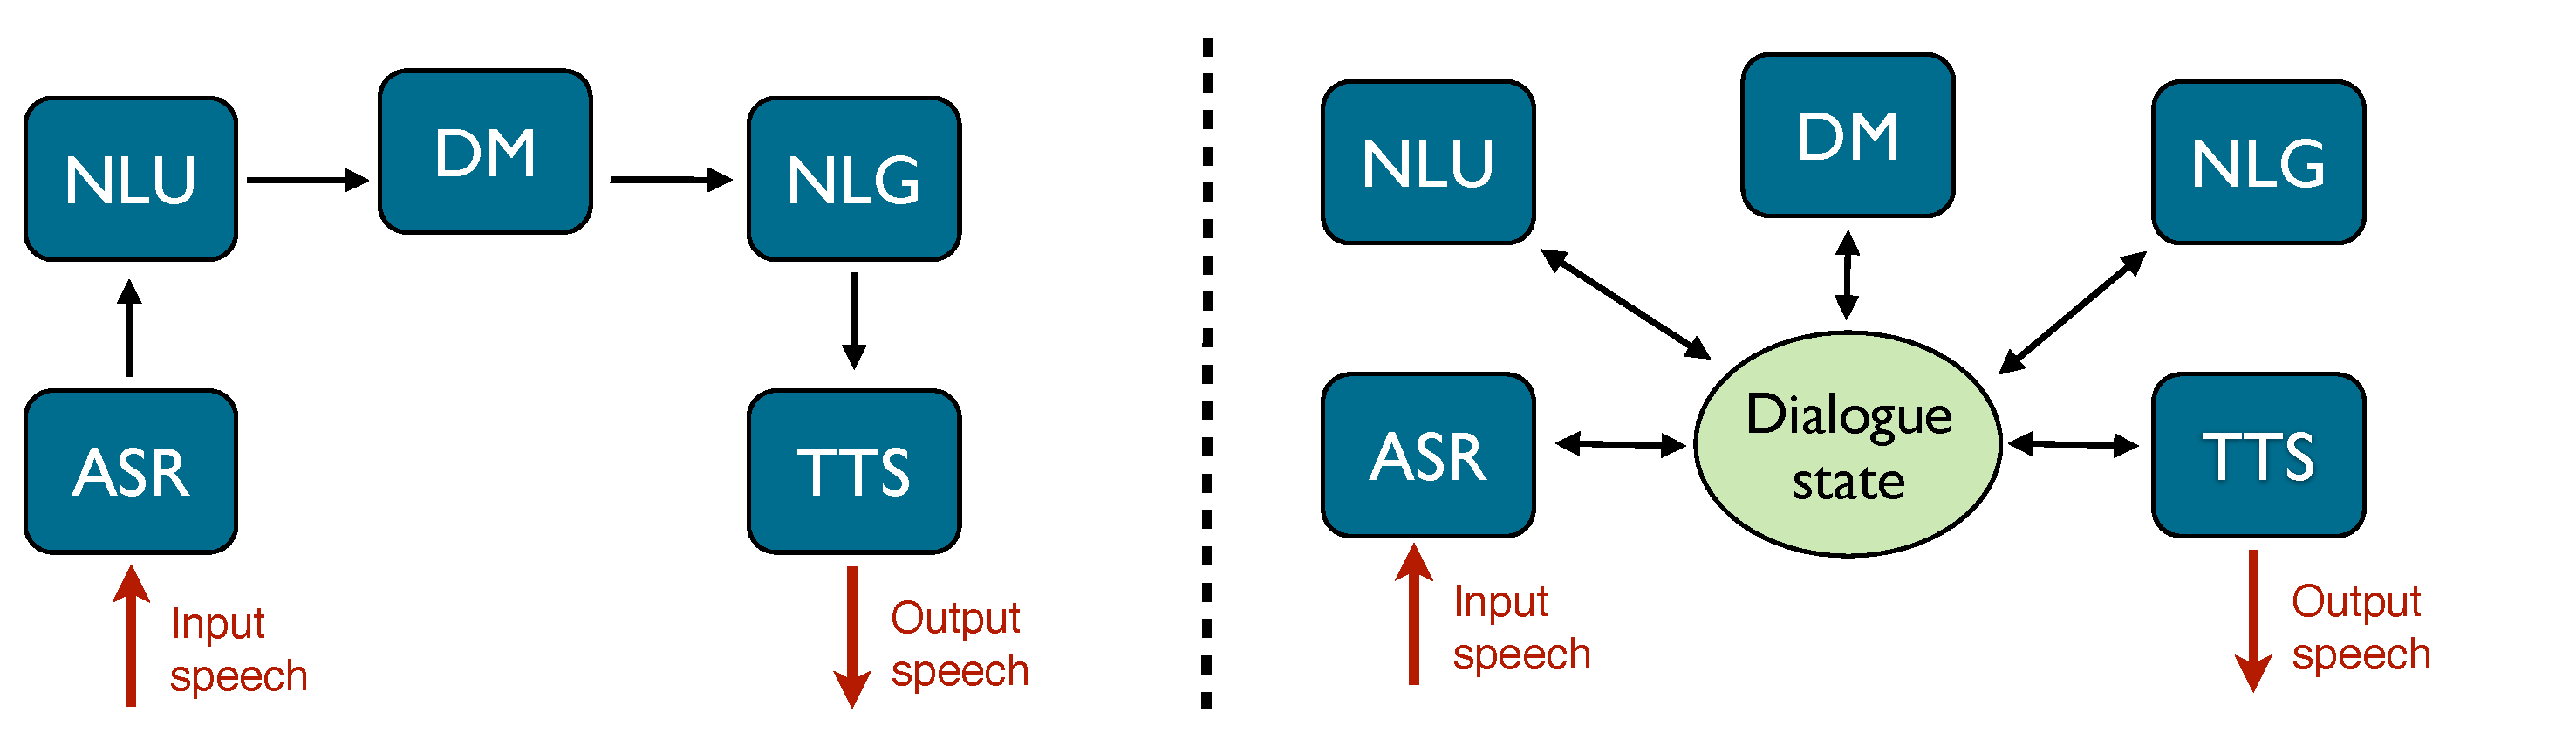
\includegraphics[scale=0.28]{imgs/architecture_comparison.pdf}
\caption{Comparison between pipeline (left) and ISU (right) system architectures.  Abbreviations: ASR = \textit{Automatic Speech Recognition}, NLU = \textit{Natural Language Understanding}, DM = \textit{Dialogue Management}, NLG = \textit{Natural Language Generation}, and TTS =\textit{Text-to-Speech Synthesis}.}
\label{fig:architecture_comp}
\end{figure}

Finally, a last aspect of dialogue system architectures that has been subject to recent research pertains to \textit{incremental processing}.  Many dialogue architectures must wait for an utterance to be fully pronounced to start its interpretation and decide on subsequent actions.  This workflow usually leads to poor reactivity and unnatural conversational behaviours.  To address this shortcoming, new architectures have been proposed to allow for incremental processing at various stages of interpretation and decision-making \citep{schlangen2009general}.\index{incremental processing}


\subsection{Components}

As we have explained, the components of a dialogue systems can typically be grouped in five important steps.  We briefly describe here the role of these components and define their respective inputs and outputs.

\subsubsection*{Speech recognition}
\index{speech recognition}
Upon detection of a new speech signal emanating from the user, the first task is to recognise the corresponding utterance. Speech recognition is responsible for converting the raw speech signal extracted from the microphones into a set of hypotheses $\tilde{u}_u$ representing the words uttered by the user. To this end, the speech signal is first converted into a digital format and split into small frames (usually 10 ms). Then, a set of acoustic features is extracted for each frame using signal processing techniques.  Once these acoustic features are extracted, two statistical models are combined to estimate the most likely recognition hypotheses: the \textit{acoustic model} and the \textit{language model}.  \index{acoustic model}\index{language model}

The acoustic model defines the observation likelihood of particular acoustic features for a given phone\footnote{A phone is an individual sound unit of speech.  Technically speaking, acoustic models are not defined over entire phones but over sub-segments, typically decomposed into three parts: beginning, middle and end.}, while the language model defines the probability of a given sequence of words. This formalisation rests on the representation of the speech recognition task as a \textit{Hidden Markov Model} (HMM)\index{Hidden Markov Model}, where the states represent the sequence of phones, and the observations are the acoustic features.  

%Given a sequence of acoustic observations $O$, the probability of a word sequence $W$ is straightforwardly derived using Bayes' rule: 
%\begin{equation}
%P(W|O) = \frac{P(O|W) P(W)}{P(O)} 
%\end{equation}
%where $P(O|W)$ is encoded by the acoustic model and $P(W)$ by the language model. $P(O)$ is a normalisation factor that can be ignored for decoding purposes. 

For the practical development of spoken dialogue systems, the most important element of a speech recogniser is the language model.  The language model effectively represents the set of utterances that can be accepted as inputs to the system (and their relative probabilities).  The model can be encoded either in the form of a hand-crafted recognition grammar, or via statistical modelling based on a particular corpus.  In the latter case, the language model typically takes the form of an N-gram model, often a bi- or tri-gram corrected with appropriate smoothing and back-off techniques  \citep{Jelinek:1998,ChenG99}.  It is also often beneficial to dynamically modify the language model during the interaction to reflect the changing context and dialogue state.  This dynamic model adaptation can notably be realised by priming the words or expressions that are most contextually relevant \citep{gruenstein2005context,ESSLLI2008-springerreprint}.

The output of the speech recogniser is typically a N-best list\index{N-best list} (or recognition lattice) representing a set of possible hypotheses for the utterance, together with their relative confidence score or probabilities.  Thus, the output of the speech recogniser is a set 
\begin{equation*}
\tilde{u}_u = \langle (u_u^{(1)}, p^{(1)}), (u_u^{(2)}, p^{(2)}), ... (u_u^{(n)}, p^{(n)})\rangle
\end{equation*}
where $u_u^{(i)}$ represents a specific recognition hypothesis and $p^{(i)}$ its corresponding probability.\footnote{In order to be proper probabilities,  the usual axioms $0 \leq p^{(i)} \leq 1$ for all $p^{(i)}$ and $\sum_{i=1}^n p^{(i)} = 1$ must be satisfied.   It should also be noted that in practice, many speech recogniser only provide raw confidence scores for their hypotheses.  Estimating the exact correspondence between these scores and meaningful probabilities is a non-trivial task that has been investigated by e.g. \cite{Williams08}.}

\subsubsection*{Speech understanding}

Once the set of recognition hypotheses for the raw utterance has been generated by the speech recogniser, the next task is to extract its semantic content.  The goal of speech understanding is to build a representation of the meaning(s) expressed by the form of a given utterance.  This task is a notoriously difficult endeavour, due to the combination of various factors. The first difficulty lies in the error rates of speech recognition, with WER (Word Error Rates) often revolving around 20 \% for many dialogue applications.\footnote{That means that one should expect one out of five words to be misrecognised by the speech recogniser.}  Many utterances also contain disfluencies of various sorts (filled pauses, repetitions, corrections etc.) and are frequently non-sentential, as already mentioned in Section \ref{non-sentential utterance}.  The combination of two phenomena seriously complicate the syntactic and semantic analysis of dialogue utterances. Finally, utterances are rife with (lexical, syntactic, referential) ambiguities\index{ambiguities} that must be resolved. 

Speech understanding can be decomposed in a number of steps.  Parsing corresponds to the task of extracting the syntactic structure of the utterance and map it into a semantic representation.  Spoken language parsing can be realised through various techniques, from keyword or concept spotting \citep{ZhangZY07,KomataniTKK01} to shallow semantic parsing \citep{Coppola:2009}, grammar-based parsing \citep{VanNoord1999} and statistical parsing \citep{He200585}.  It has been shown useful to apply upstream preprocessing techniques to correct some speech errors \citep{Ringger:1996} and filter out disfluencies \citep{Johnson:2004}. In addition, speech understanding might also need to resolve referring expressions \citep{Funakoshi:2012}.  And finally, the dialogue act associated with the utterance must be determined \citep{stolcke2000,Keizer2007}. \cite{demori2008} provides a survey of the various models and techniques used in the field of spoken language understanding. 

Given speech recognition hypotheses $\tilde{u}_u$ provided as inputs, and possibly a representation of the dialogue history and external context, the task of speech understanding is to extract a corresponding set of dialogue act hypotheses $\tilde{a}_u$ defined as: \begin{equation*}
\tilde{a}_u = \langle (a_u^{(1)}, p^{(1)}), (a_u^{(2)}, p^{(2)}), ... (a_u^{(n)}, p^{(n)})\rangle
\end{equation*}
where $a_u^{(i)}$ represents a dialogue act hypothesis, usually represented in a logical form with various predicates and arguments, and $p^{(i)}$ its corresponding probability.

\subsubsection*{Dialogue management}
\index{dialogue management}

Dialogue management occupies a central stage in spoken dialogue systems.  As we already mentioned in the introductory chapter, dialogue management serves a double role.  The first task of the dialogue manager is to maintain a representation of the current dialogue state\index{dialogue state} and update it as new information becomes available\index{dialogue state update}.  This dialogue state should encode every information that is of general relevance for the dialogue system.  In addition to the last dialogue act from the user, the dialogue state can therefore also include the previous dialogue history (as a temporally ordered sequence of dialogue acts performed by the conversational partners), the current conversational floor, the status of the task(s) to fulfil, and various features describing the context of the interaction.  Furthermore, the dialogue state can also include information that is indirectly inferred from the individual observations provided by the other modules. In particular, many dialogue systems include a variable that explicitly encode the assumed user intention.  This user intention, although never directly observed, can often be derived from the user inputs through a sequence of reasoning steps.  Similarly, the dialogue state can also define features that attempt to characterise the user and her/his preferences.\index{user model} Depending on the theoretical premises chosen by the system designer, the dialogue state can either be encoded as a fully observable data structure, or can be extended to explicitly represent partial observability through the definition of probability distributions on the values of the state variables. 

The second task of dialogue management is to make decisions based on this dialogue state.  This task is often called \textit{action selection}. \index{action selection}The decision pertains to the next action to perform by the system, and can be either a communicative action (e.g. a piece of information to communicate, a question to task, a grounding signal to convey) or an external action (e.g. a physical movement for a robot or a database manipulation for a booking system). Action selection can either be directly hand-crafted by the system designer (through e.g. a function directly associating each state with a particular decision) or be the result of forward planning.  In the latter case, the dialogue manager must consider various alternatives and select the action that is expected to be ``optimal'' (that is, which will yield the highest utility for the system) given the current state.  This planning process can be either done online or be precompiled in advance through offline techniques.

The outcome of the dialogue management step is two-fold: (1) an updated dialogue state $s'$ that reflects the observations received as inputs (user dialogue acts, contextual changes etc.), and (2) a selected system action denoted as $a_m$ (the $m$ subscript standing for ``machine'').  This system action can correspond to a communicative action, an external action, or be null (i.e. no action).  As for the user act $a_u$, the system action $a_m$ is often encoded in a logical format with predicates and arguments. 

Section \ref{sec:dm} describes in more detail the various approaches and techniques that have been proposed in the literature to tackle the dialogue management problem. 

\subsubsection*{Generation}
\index{natural language generation}
Assuming the selected system action $a_m$ relates to a communicative action, the following step is to find the best linguistic realisation for the abstract goal defined in $a_m$.  

%The dialogue manager selects \textit{what} to say, a the role of the generation component is to find \textit{how} to say it. 

As for speech understanding, a variety of techniques can be adopted, from shallow generation strategies based on canned sentences or templates to more more sophisticated approaches based on sentence planning \citep{Stone2003,koller-stone:2007}.  More recently, statistical methods have also been fruitfully pursued in enhance the robustness and user-adaptivity of the generation algorithms \citep{Rieser:2010,DethlefsC11}. 

The inputs of the generation module are the selected system action $a_m$ and optionally the features defined in the dialogue state $s$ (e.g. the user model and the external context). Given this information, the generation module will produce a corresponding user utterance denoted $u_m$.  In the case of multimodal systems, the module might also deliver realisations for other modalities than the speech channel, such as gestures or facial expressions.

\subsubsection*{Speech synthesis}
\index{text-to-speech synthesis}\index{speech synthesis}
The final step of the processing cycle is to synthesise the utterance in a speech waveform --  a procedure called \textit{text-to-speech synthesis}.  This mapping is performed in two consecutive stages.  First, the words of the utterance are converted into a phonemic representation. This conversion involves various processing operations related to text normalisation, phonetic and prosodic analysis.  Once this conversion is completed, the resulting phonemic representation is fed into a synthesiser in charge of producing the actual waveform. Two alternative families of methods exist to perform this synthesis: \textit{concatenative synthesis} glues together pre-recorded units of speech (taken from a speech database), while \textit{formant and articulatory synthesis} generate sounds using explicit acoustic models of the vocal tract. Most dialogue systems in current use rely on concatenative synthesis, and in particular unit selection \citep{hunt1996}. 

\subsection{Applications}

Spoken dialogue systems have a wide variety of applications, ranging from academic research prototypes to mature commercial products. The first applications can be found in telephone-based systems for information access and service delivery.  A large variety of systems have been developed in this area, for applications as diverse as automated call-routing \citep{GorinRW97}, weather information \citep{jupiter}, travel planning \citep{walker2001}, bus schedule delivery \citep{RauxLBBE05} or tourist information \citep{lemon2006}.  The recent emergence of smartphones also led to the development of new voice interfaces for multimodal local search \citep{EhlenJ13}, cross-lingual communication \citep{yochina} and even pedestrian exploration  \citep{janarthanam2012integrating}.  Many of these ideas have found their way into commercial products, as evidenced by the success of applications such as Apple's Siri, Nuance's Dragon Go! and Google Now. 

Spoken dialogue systems can also be fruitfully applied in domains where the use of touch interfaces and screens should be avoided because it is impractical or dangerous.  This is notably the case for in-car navigation systems where voice interfaces are to be preferred for safety reasons \citep{cumove,CastronovoMPM10}.  Similarly, the recent trends towards ubiquitous computing and ``ambient'' intelligence for smart home environments offer promising applications of dialogue system technology \citep{vipperla2009a,ambient2010}.

Spoken dialogue systems are applied to increasingly complex and open-ended interaction domains, where the artificial agent is no longer a mere executor of user commands, but becomes more of a collaborator or intelligent assistant.  Conversational interfaces have notably developed in the healthcare sector to monitor (and hopefully improve) the health condition and fitness of patients through interactive dialogues \citep{BickmoreG06,Stahl:2009,MorbiniFDSTR12}.  Substantial research has also been devoted into the development of interactive tutoring assistants in various learning settings \citep{ChiVLJ11,Dzikovska:2011,jan2011,TraumAAFGKLNS12}. 

Finally, dialogue systems form an integral part of many robotic systems.  Robots are deployed in increasingly social environments, such as homes, offices, schools and hospitals.  As a consequence, many of these robots require the ability to interact with their human users through a simple and intuitive interface such as speech.  Human-robot interaction is an active area of research and has focussed on multiple aspects such as situated dialogue processing \citep{CantrellSSW10,cosybook:dialogue}, adaptivity \citep{DoshiR08}, symbol grounding \citep{Roy05,lemaignan2012} and multimodal interaction \citep{stiefelhagen2004,salem2012,MirnigWSMGBGT13}.

\section{Dialogue Management}
\label{sec:dm}

Various approaches have been proposed to formalise the dialogue management problem.

\note{such as an Attribute-Value Matrix (AVM, encoding of the user intention}
information state update
\subsection{Hand-crafted approaches}

Some topics investigated in this paradigm are the semantic and pragmatic interpretation of dialogue moves \citep{ThomasonManuscript-THOEUA,Ginzburg2012}, the rhetorical structure of dialogue \citep{0521659515}, or the use of plan-based reasoning to infer the user intentions \citep{Allen1980,Litman87}.  These approaches are able to provide detailed analyses of various dialogue behaviours, but they generally assume complete observability of the dialogue context and provide only a very limited account (if any) of uncertainties.

\citep{Grosz:1986} about plan-based approach. 

\note{Finite-state automata, frame-based, logical reasoning, etc.}

\subsection{Statistical approaches}


This is typically done by representing the dialogue domain as a Markov Decision Process (MDP) or Partially Observable Markov Decision Process (POMDP) and subsequently estimating the parameters of these models from data \citep{Supelec270}. 

 related to partial observability (noisy spoken inputs, unknown user intentions) and stochastic action effects (the user behaviour can be hard to predict). 
 
  Probabilistic modelling techniques must however face two important challenges. The most pressing issue is the paucity of appropriate data sets.  Statistical models often require large amounts of training data to estimate their parameters. Unfortunately, real interaction data is scarce, expensive to acquire, and difficult to transfer from one domain to another.  Moreover, many domains exhibit a rich internal structure with multiple tasks to perform, sophisticated user models, and a complex, dynamic context.  In such settings, the dialogue system might need to track a large number of variables in the course of the interaction, which quickly leads to a combinatorial explosion of the state space.  
  
\note{MDP and POMDPs}

\section{Summary}

\note{5 points about dialogue? uncertain, structured, contextual, goal-driven, collaborative}

%They also continuously seek to predict what their interlocutor is going to say or talk about next, based on the current context \citep{VanBerkum2005}.  They cover a wide range of behavioural levels, from low-level imitation mechanisms to high-level alignment of semantic representations \citep{Garrod2009}.


\note{not said: predictions, incrementality, embodiment and situatedness, conversation structure}

\begin{table}[h]
\begin{center}
\begin{tabular}{|p{25mm}|p{25mm}|p{20mm}|p{25mm}|p{30mm}|} \hline
\centering \vspace{0mm} Approach &  \centering \vspace{-1mm} State representation &  \centering \vspace{-1mm} Partial observability &  \centering \vspace{0mm}State update &  \vspace{0mm}\centerline{Action selection} \\ \hline
Finite State Automata & State symbol & no & Traversal of matching edge & Selection of action associated with current node \\ 
\end{tabular}
\end{center}
\caption{Comparison of dialogue management approaches.}
\label{table:approaches}
\end{table}